\documentclass[FIPLY_base.tex]{subfiles}

%\author{Gerald Irsiegler}
%\date{26. Februar 2016}

\begin{document}

\subsection{Datenbank}
\subsubsection{Beschreibung}
In der Datenbank werden alle für die Applikation essentiellen Daten gespeichert.

\subsubsection{SQLite}
SQLite ist eine open-source Library, sie implementiert ein unabhängiges, serverloses, ''zero-configuration'' und transaktionales SQL-database-engine [\citetitle{dbSQLite}\cite{dbSQLite}]. SQLite ist die beste Lösung da die Daten nur in einer Applikation verwendet werden.

\subsubsection{ContentProvider}
Der ContentProvider kapselt den Datenzugriff vom lokalen Speicher des Gerätes, er wird hauptsächlich benützt falls Daten zwischen Applikationen ausgetauscht werden. 

\subsubsection{Zugriff auf die Daten}


\paragraph{Datenbank Architektur}\ \\
Der Zugriff auf die abgespeicherten Daten erfolgt über 4 Schichten:

\begin{figure}[H]
	\begin{subfigure}[b]{0.3\textwidth}
	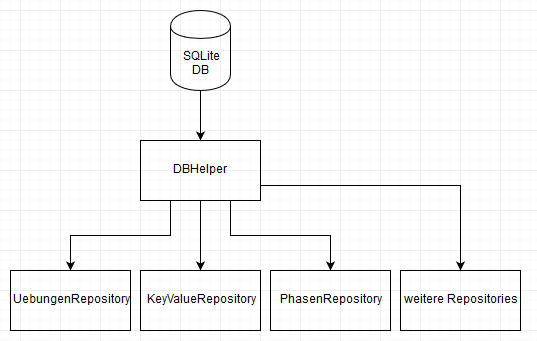
\includegraphics[scale=0.4]{img/Database_architecture}
	\end{subfigure}
	\hfil
	\caption{Die Datenbank-Architektur.}
\end{figure}

\paragraph{Phsysische Ebene}\ \\
Alle Daten werden im lokalen Speicher des Mobilgerätes abgelegt und persistiert. Die Speicherung übernimmt das DBMS von SQLite.

\paragraph{Datenbankobjekt}\ \\
Das Datenbankobjekt ist jenes, welches im lokalen Speicher abgelegt ist und von der nächsten Schicht instanziert wird. Es enthält die Informationen über alle in der Datenbank abgespeicherten Daten und erlaubt es auf diese zuzugreifen.

\paragraph{DB Helper}\ \\
Der DB Helper kapselt das Datenbankobjekt und stellt es den Repositories zur Verfügung. Der DB Helper ist als Singleton implementiert und wird in den Repositories instanziert.


\newpage
\paragraph{Repositories}\ \\
Die Repositories dienen als Puffer zwischen dem Datenbankobjekt und der Businesslogik.
Jedes Repository ist als Singleton implementiert und um darauf zugreifen zu können muss es vorerst im Code instanziert werden.
\ \\
\begin{lstlisting}[caption={Repository wird instanziert.},label=DescriptiveLabel]
Repository repository = Repository.getInstance();
\end{lstlisting}

\ \\
In den Repositories muss das Datenbankobjekt mithilfe des DB Helpers instanziert werden ...
\ \\
\begin{lstlisting} [caption={Das Datenbankobjekt db wird instanziert über den FiplyDBHelper},label=DescriptiveLabel]
    SQLiteDatabase db = getWritableDatabase();

    private SQLiteDatabase getWritableDatabase() {
        if (repoContext == null) 
            throw new IllegalStateException();
	  
        return FiplyDBHelper.getInstance(repoContext)
			      	  		        .getWritableDatabase();
    }
\end{lstlisting}
\ \\
... um über dieses Objekt dann mithilfe von SQL-Statements auf die Daten zugreifen bzw. die Daten manipulieren zu können.
\ \\
\begin{lstlisting} [caption={db wird instanziert und ein SQL Statement wird ausgeführt.},label=DescriptiveLabel]
SQLiteDatabase db = getWritableDatabase();

return db.query("SQL-STATEMENT");
\end{lstlisting}

\ \\
Folgende Repositories sind in der Applikation vorhanden:
\begin{itemize}
\item Instruktionen-Repository
\item Key-Value-Repository
\item Phasen-Repository
\item Plan-Repository
\item Playlist-Songs-Repository
\item Statistik-Repository
\item Uebungen-Repository
\end{itemize}

\newpage
\subsubsection{Contract}
Der Contract ist eine Datei in welcher die Metadaten der Datenbank zu finden sind.
Dieser "Vertrag" existert um den makellosen Zugriff auf die Datenbank sicherzustellen.
Für jede Tabelle in der Datenbank wird im Contract eine eigene Klasse angelegt, diese beinhaltet den Tabellennamen und die Namen aller ihrer Attribute als strings.
\begin{lstlisting}[caption={Eine Contract Klasse, mit allen Metadaten.},label=DescriptiveLabel]
    public static final class UebungenEntry implements BaseColumns {
        public static final String TABLE_NAME = "uebungen";
        public static final String COLUMN_ROWID = "_id";
        public static final String COLUMN_NAME = "name";
        public static final String COLUMN_MUSKELGRUPPE = "muskelgruppe";
        public static final String COLUMN_BESCHREIBUNG = "beschreibung";
        public static final String COLUMN_ANLEITUNG = "anleitung";
        public static final String COLUMN_SCHWIERIGKEIT = "schwierigkeit";
        public static final String COLUMN_VIDEO = "video";
        public static final String COLUMN_EQUIPMENT = "equipment";
    }
\end{lstlisting}

\end{document}
